\chapter{Results}
\label{ch:results}
The Anaconda Platform is used for overall design and implementation on the MAC Book Pro. We created six Python files that show the overall changes from 5 minutes, 1 hour, and 1 day for the ARIMA-ANN Hybrid and TNN algorithms. The design includes argument analysis for code execution for each type of firm, and the calling feature is more user-friendly. The ARIMA-ANN hybrid design was carried out with ARIMA parameters (2,1,3), and for TNN, we used 2-layer Dense modeling for encoder and decoder, as shown in Algorithm 1. The total experiment on timeseries prediction was carried out based on the numerous functional elements indicating the time features of the Yahoo finance stocks for the advancement.The goal of this paper is to provide a solution that will predict Yahoo's total stock price, suggesting the best prediction method.

The design models are executed in two stages for each form of effective inquiry, one representing the prediction time values for the stocks and the other reflecting the overall effective loss observed variation on each type of company, assuring the corrected next day projected value.

\section{Comparision of Algorithms}
Based on the predicted values accuracy,  calculated mean square error and considering the time taken to calculate the stock values of the given input company Transformer neural network performs better in the current scenario in both predicting the values and time taken for calculations with less RMSE value compared to ARIMA-ANN hybrid. ARIMA-ANN hybrid also performs well to calculate the stock values but while training ANN part of the model, it consumes more time for calculations. 
In light of this, we may conclude that the Transformer neural network outperformed all others in terms of stock price prediction for a particular ticker.

The following images are the results from the model regarding predicting the values of next day stock.

\begin{figure}[ht]
    \centering
    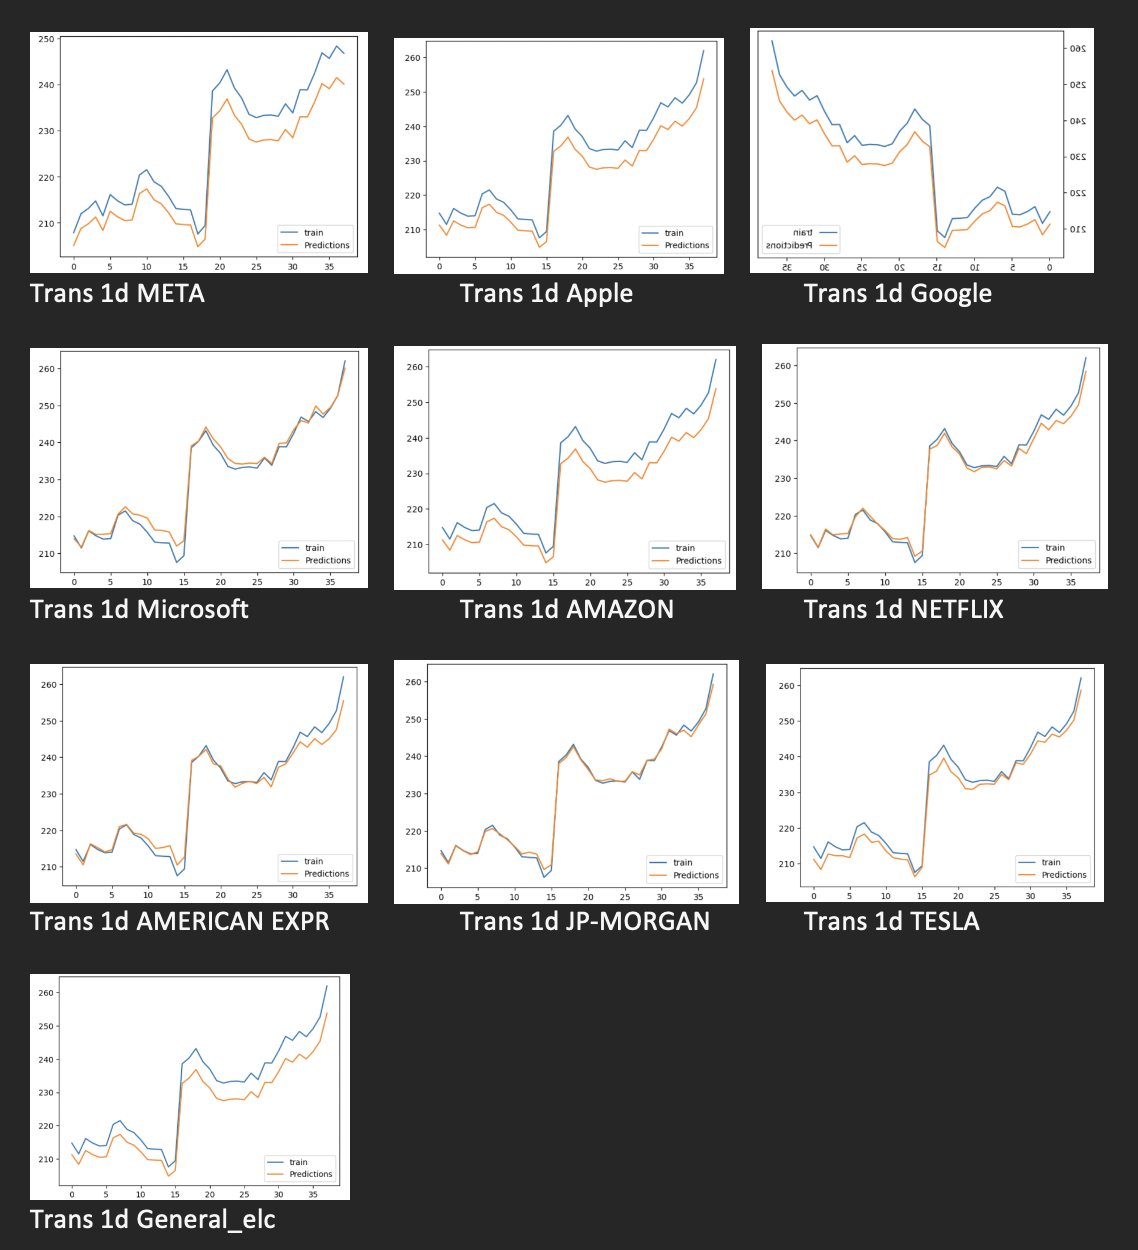
\includegraphics[scale=0.2]{figures/Trans 1d.png}
    \caption{Representing the overall actual and predicted values for Close stock for TNN algorithms with time period as 1d.}
    \label{fig:chart_b}
\end{figure}
\textbf 

\begin{figure}[ht]
    \centering
    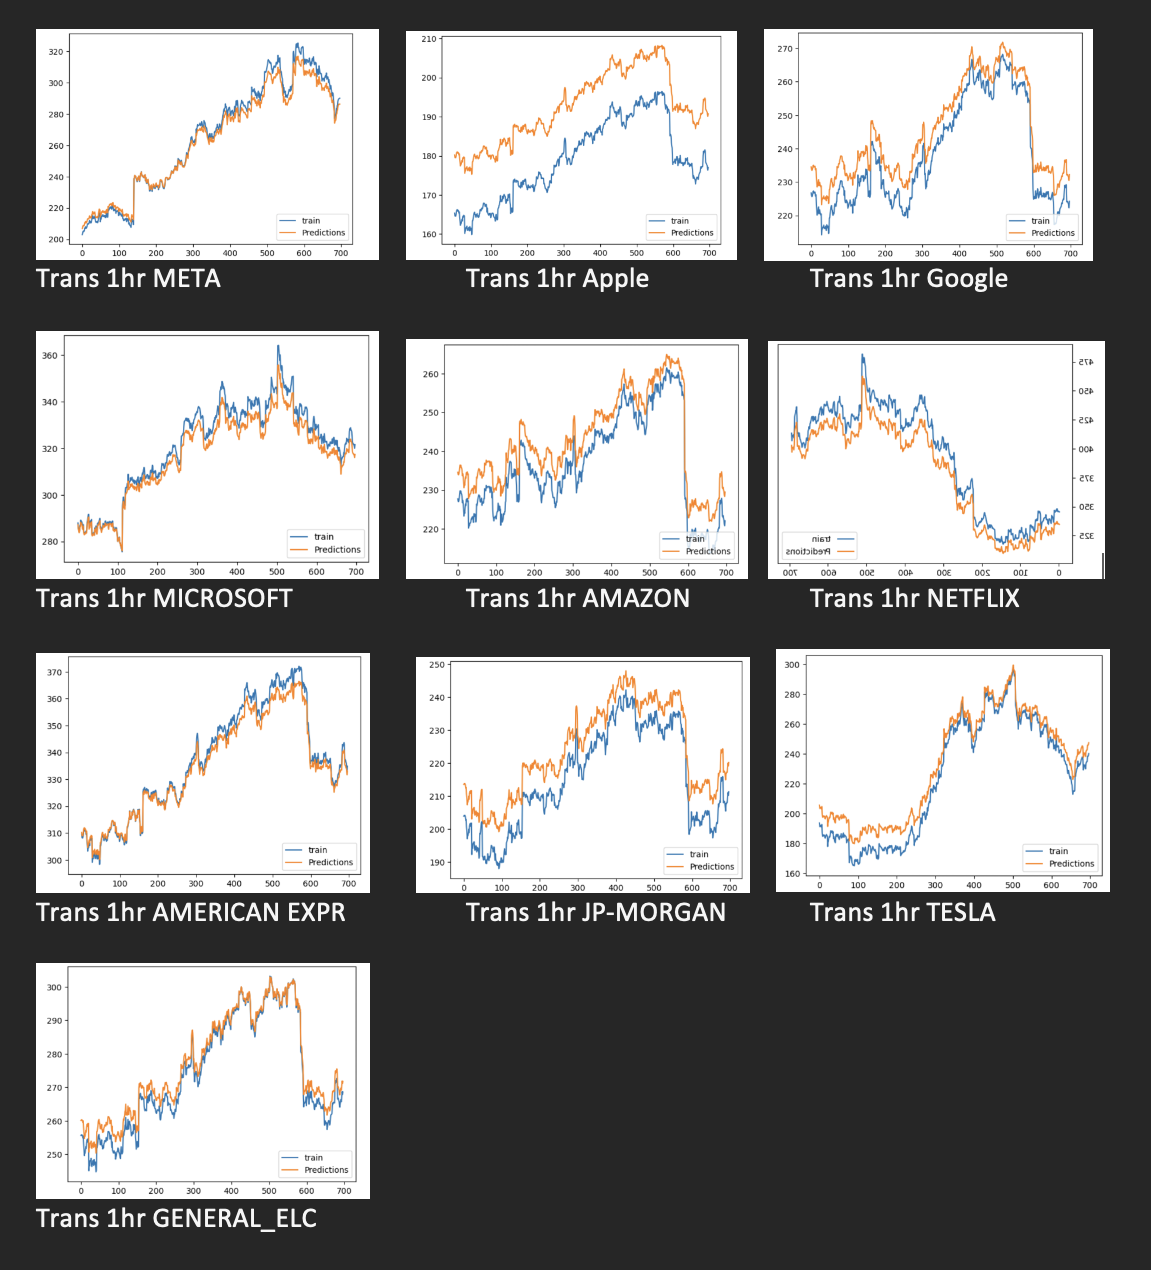
\includegraphics[scale=0.2]{figures/Trans 1hr.png}
    \caption{Representing the overall actual and predicted values for Close stock for TNN algorithms with time period as 1hr.}
    \label{fig:chart_a}
\end{figure}

\begin{figure}[ht]
    \centering
    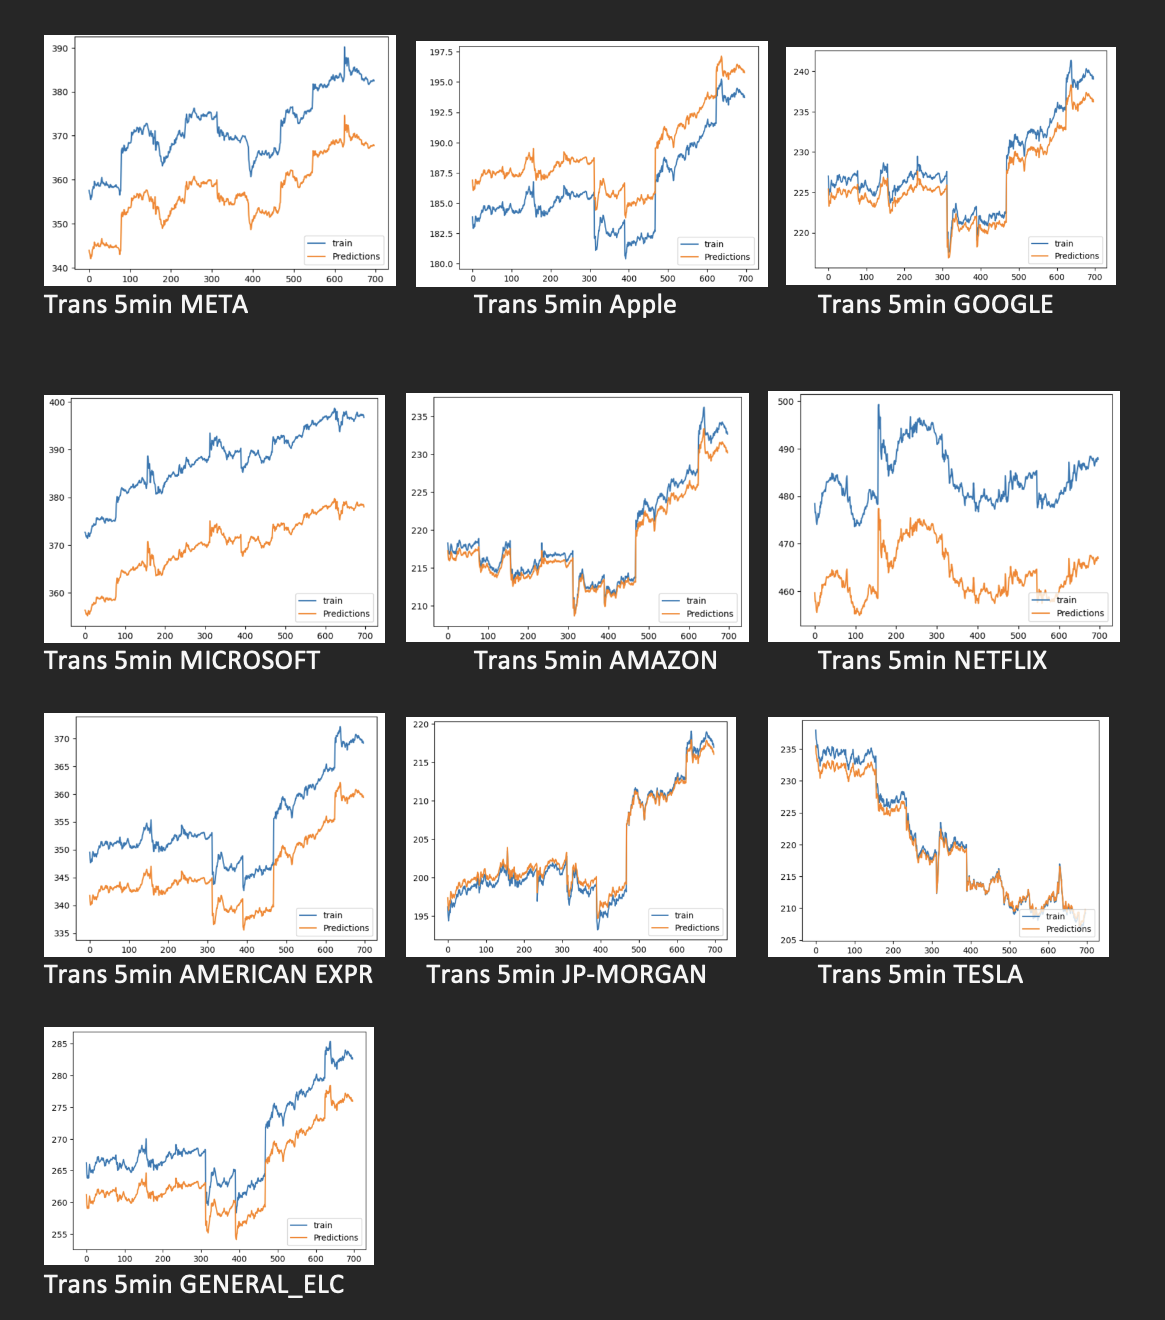
\includegraphics[scale=0.2]{figures/Trans 5min.png}
    \caption{Representing the overall actual and predicted values for Close stock for TNN algorithms with time period as 5min.}
    \label{fig:chart_c}
\end{figure}

\begin{figure}[ht]
    \centering
    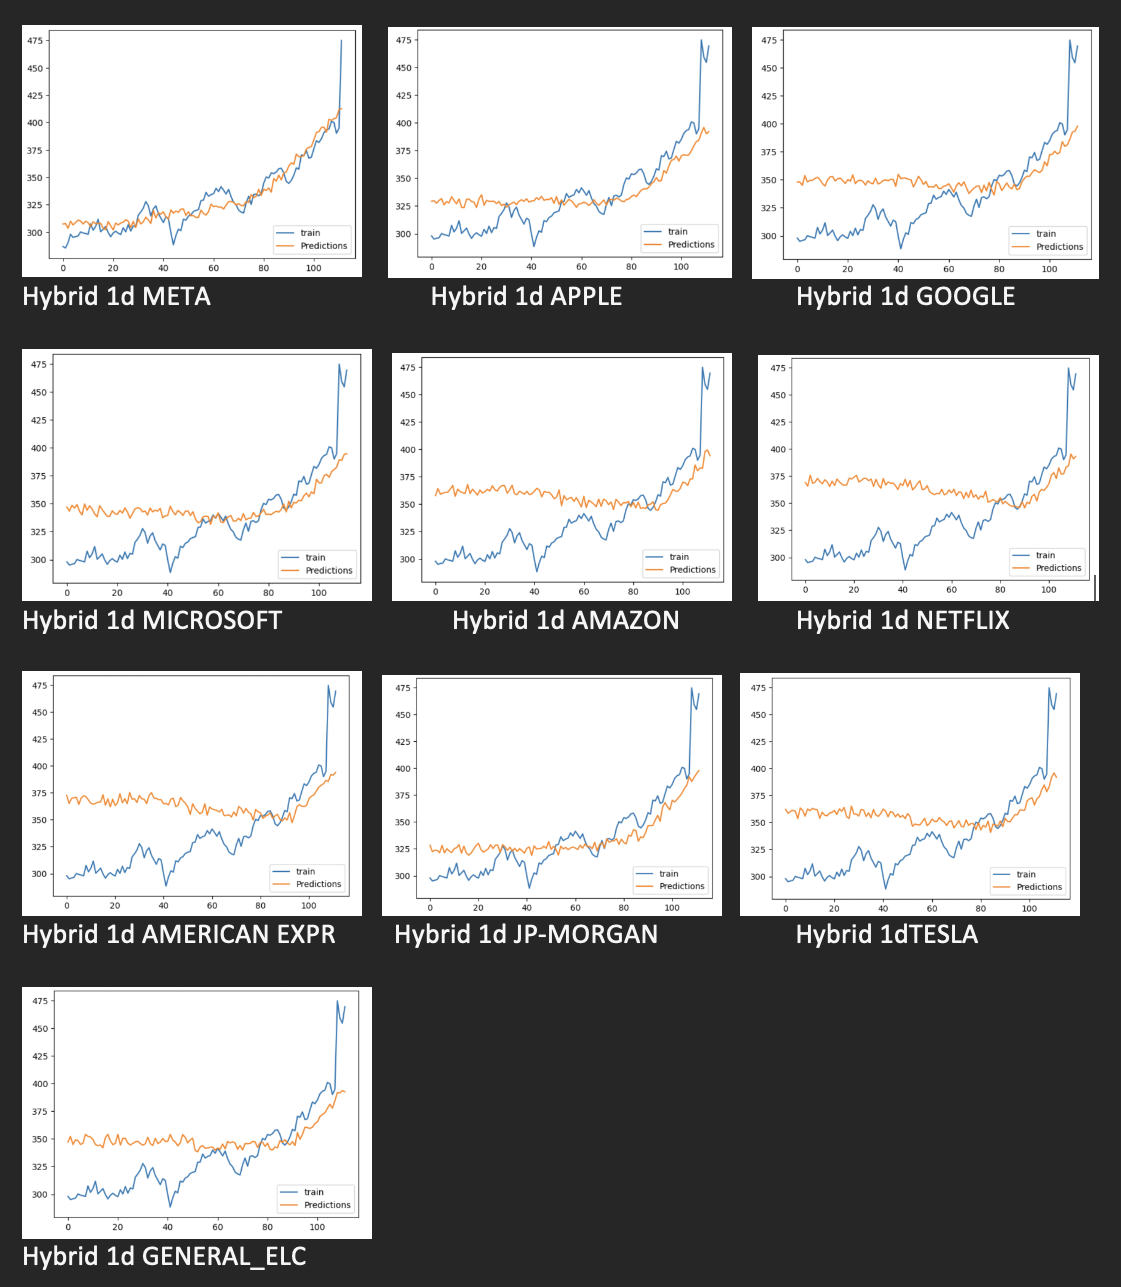
\includegraphics[scale=0.2]{figures/Hybrid 1d.png}
    \caption{Representing the overall actual and predicted values for Close stock for ARIMA-ANN algorithms with time period as 1day.}
    \label{fig:chart_e}
\end{figure}

\begin{figure}[ht]
    \centering
    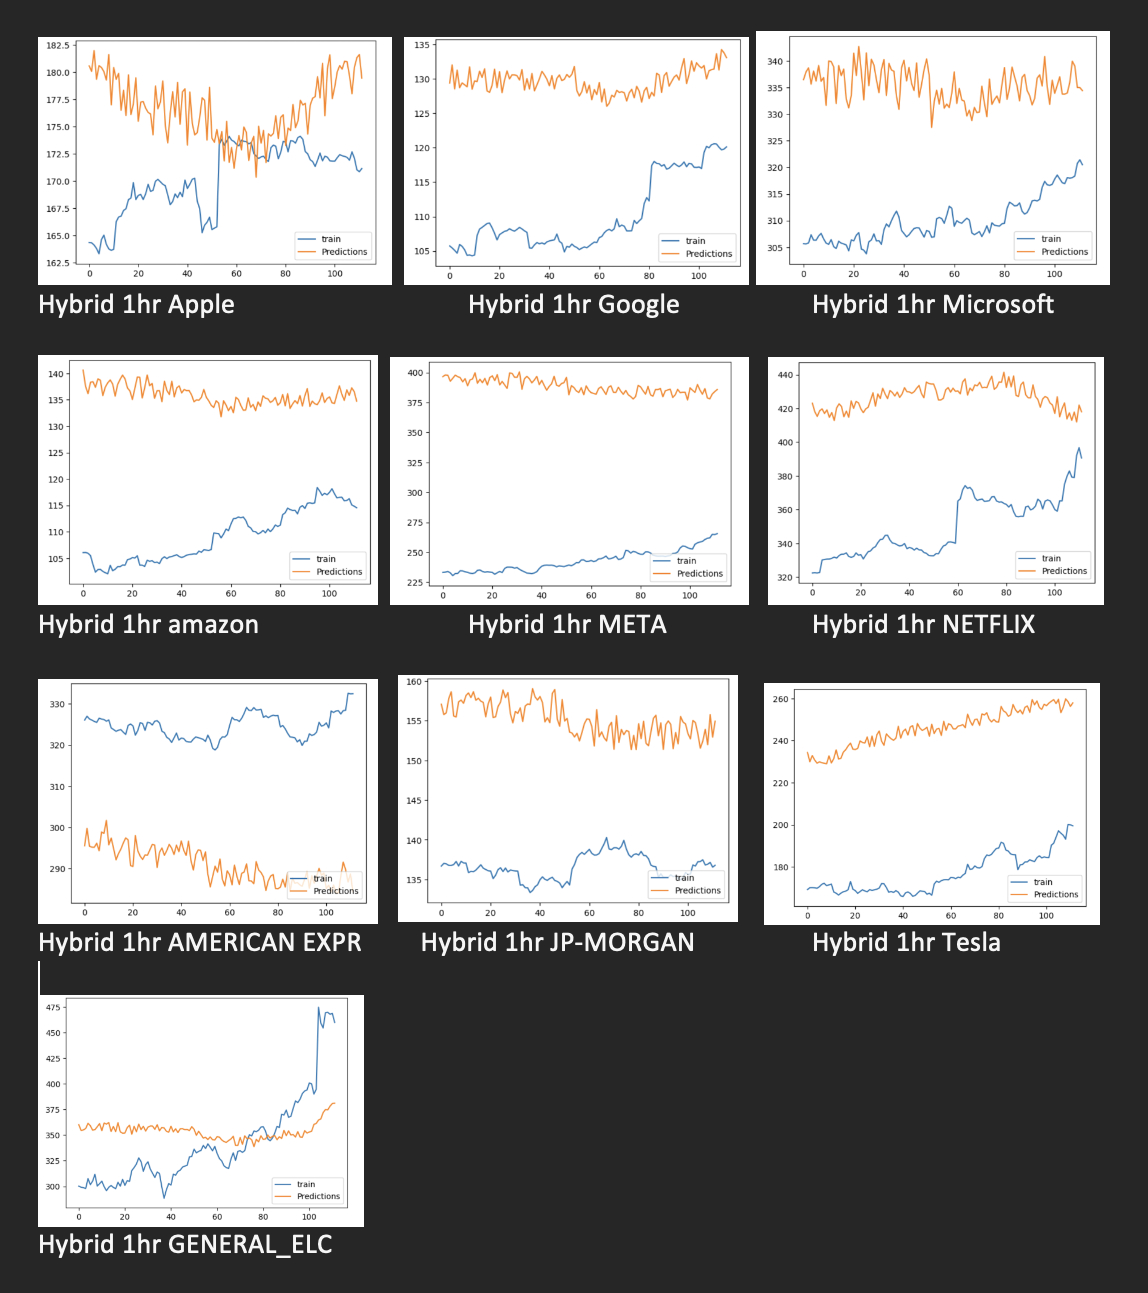
\includegraphics[scale=0.2]{figures/Hybrid 1hr.png}
    \caption{Representing the overall actual and predicted values for Close stock for ARIMA-ANN algorithms with time period as 1hr.}
    \label{fig:chart_d}
\end{figure}

The overall differences in the forecasts between the ARIMA-ANN and TNN outcomes are shown for every iteration throughout the designated time frame. The ARIMA-ANN and TNN model designs have undergone several modifications, and the interpolation methods show improvements in the overall prediction procedure, which favors TNN over ARIMA-ANN. In order to guarantee the effective loss for the design, our TNN design made use of the Dense layer, which has various functional capabilities providing overall alterations in the attentions, activation, and feedforwarding classes.

Figure 5.1 shows the total forecast values for the 10 tickers under consideration, providing a broad overview of how the predictions and actual values differ. The overall charting of these characteristics is dependent on the multi-objective function post-prediction interpolation based on the prediction with various constraints on each and every sample that is taken into consideration.


